\documentclass[12pt,a4paper]{article}
\usepackage[utf8]{inputenc}
\usepackage[T1]{fontenc}
\usepackage{graphicx}
\usepackage{float}
\usepackage{amsmath}
\usepackage{amsfonts}
\usepackage{amssymb}
\usepackage{geometry}
\usepackage{hyperref}
\usepackage{booktabs}
\usepackage{array}
\usepackage{subcaption}
\usepackage{listings}
\usepackage{xcolor}
\usepackage{fancyhdr}
\usepackage{titlesec}

% Page geometry
\geometry{margin=1in}

% Header and footer
\pagestyle{fancy}
\fancyhf{}
\rhead{ARN Duck Species Classification Project}
\lfoot{\today}
\rfoot{\thepage}

% Title formatting
\titleformat{\section}{\Large\bfseries}{\thesection}{1em}{}
\titleformat{\subsection}{\large\bfseries}{\thesubsection}{1em}{}
\titleformat{\subsubsection}{\normalsize\bfseries}{\thesubsubsection}{1em}{}

% Code listing style
\lstset{
    basicstyle=\ttfamily\small,
    breaklines=true,
    frame=single,
    backgroundcolor=\color{gray!10}
}

% Hyperref settings
\hypersetup{
    colorlinks=true,
    linkcolor=blue,
    filecolor=magenta,
    urlcolor=cyan,
    pdftitle={ARN Duck Species Classification Project},
    pdfauthor={Kilian Froidevaux and Bovard Nicolas}
}

\title{\textbf{ARN Duck Species Classification Project}\\
\large Object Recognition in the Wild using Convolutional Neural Networks}
\author{Kilian Froidevaux and Bovard Nicolas\\HEIG-VD - Practical Work 05}
\date{\today}

\begin{document}

\maketitle

\tableofcontents
\clearpage

\section{Introduction}

The goal of this project is to classify images of ducks into different species using a Convolutional Neural Network (CNN). The dataset consists of images of ducks taken in various locations and the classification task is to identify the species of each duck.

The idea is that the user can take a picture of a duck with their phone (bad quality picture) and the model will classify it into one of the species (on a predefined list). The model should be lightweight enough to run on a mobile device, so we will use transfer learning with MobileNetV2.

\section{The Problem}

The dataset consists of images of ducks taken in various locations with the phone and taken by us. The species to classify are:

\begin{itemize}
    \item \textit{Canard colvert mâle} (Male Mallard)
    \item \textit{Canard colvert femelle} (Female Mallard)
    \item \textit{Foulque macroule} (Eurasian Coot)
    \item \textit{Grèbe huppé} (Great Crested Grebe)
    \item \textit{Autre} (Other)
\end{itemize}

The first idea was to classify the species of ducks that are commonly found in Switzerland. The dataset is small, with only a few images per species, which makes it a challenging task.

Initially, we wanted to classify more species of ducks (like \textit{Cygne Tuberculé} and \textit{Harle Bièvre}), but due to the limited number of images available, we had to reduce the number of species to five. The dataset is unbalanced, with some species having more images than others.

We will still test the model performance on these 2 more species to see its performance but since we had a hard time to find a working model, we decided to focus on the five species listed above.

Below are the class weights (1/distribution) to show how class imbalance is handled:

\begin{figure}[H]
    \centering
    \includegraphics[width=0.8\textwidth]{../../output/best_model_duck_classification_f1_optimized_20250608_195712/plots/class_weights.png}
    \caption{Class weights distribution showing dataset imbalance}
    \label{fig:class_weights}
\end{figure}

One thing to note is that for duck species with different features between sexes, we split them into two classes: \textit{Canard colvert mâle} and \textit{Canard colvert femelle} to help the model distinguish between them (it also gives one more feature to the application).

\section{Data Preparation}

\subsection{Data Query}

The dataset was created by taking pictures of ducks in various locations. The images were taken with a phone camera, which means that the quality of the images is not always optimal. The images were taken in various locations and conditions, which adds to the complexity of the classification task.

We cropped the images with multiple ducks in the same picture to focus on the duck we want to classify.

We also took pictures of other species and background without ducks to help the model distinguish between the species and the background so that it could classify these images as \textit{Autre}.

\subsection{Data Preprocessing}

We resized the images to a fixed size of 224×224 pixels to match the input size of the MobileNetV2 model. We also normalized the pixel values to be in the range [0, 1] by dividing by 255.

\subsection{Data Augmentation}

Since the dataset is small, we used data augmentation techniques to artificially increase the size of the dataset. We applied most of the data augmentation techniques that we found such as:

\begin{itemize}
    \item Random rotation
    \item Random horizontal/vertical flip
    \item Random brightness adjustment
    \item Random contrast adjustment
    \item Random saturation
    \item Random hue
\end{itemize}

Below is an example of such augmentations:

\begin{figure}[H]
    \centering
    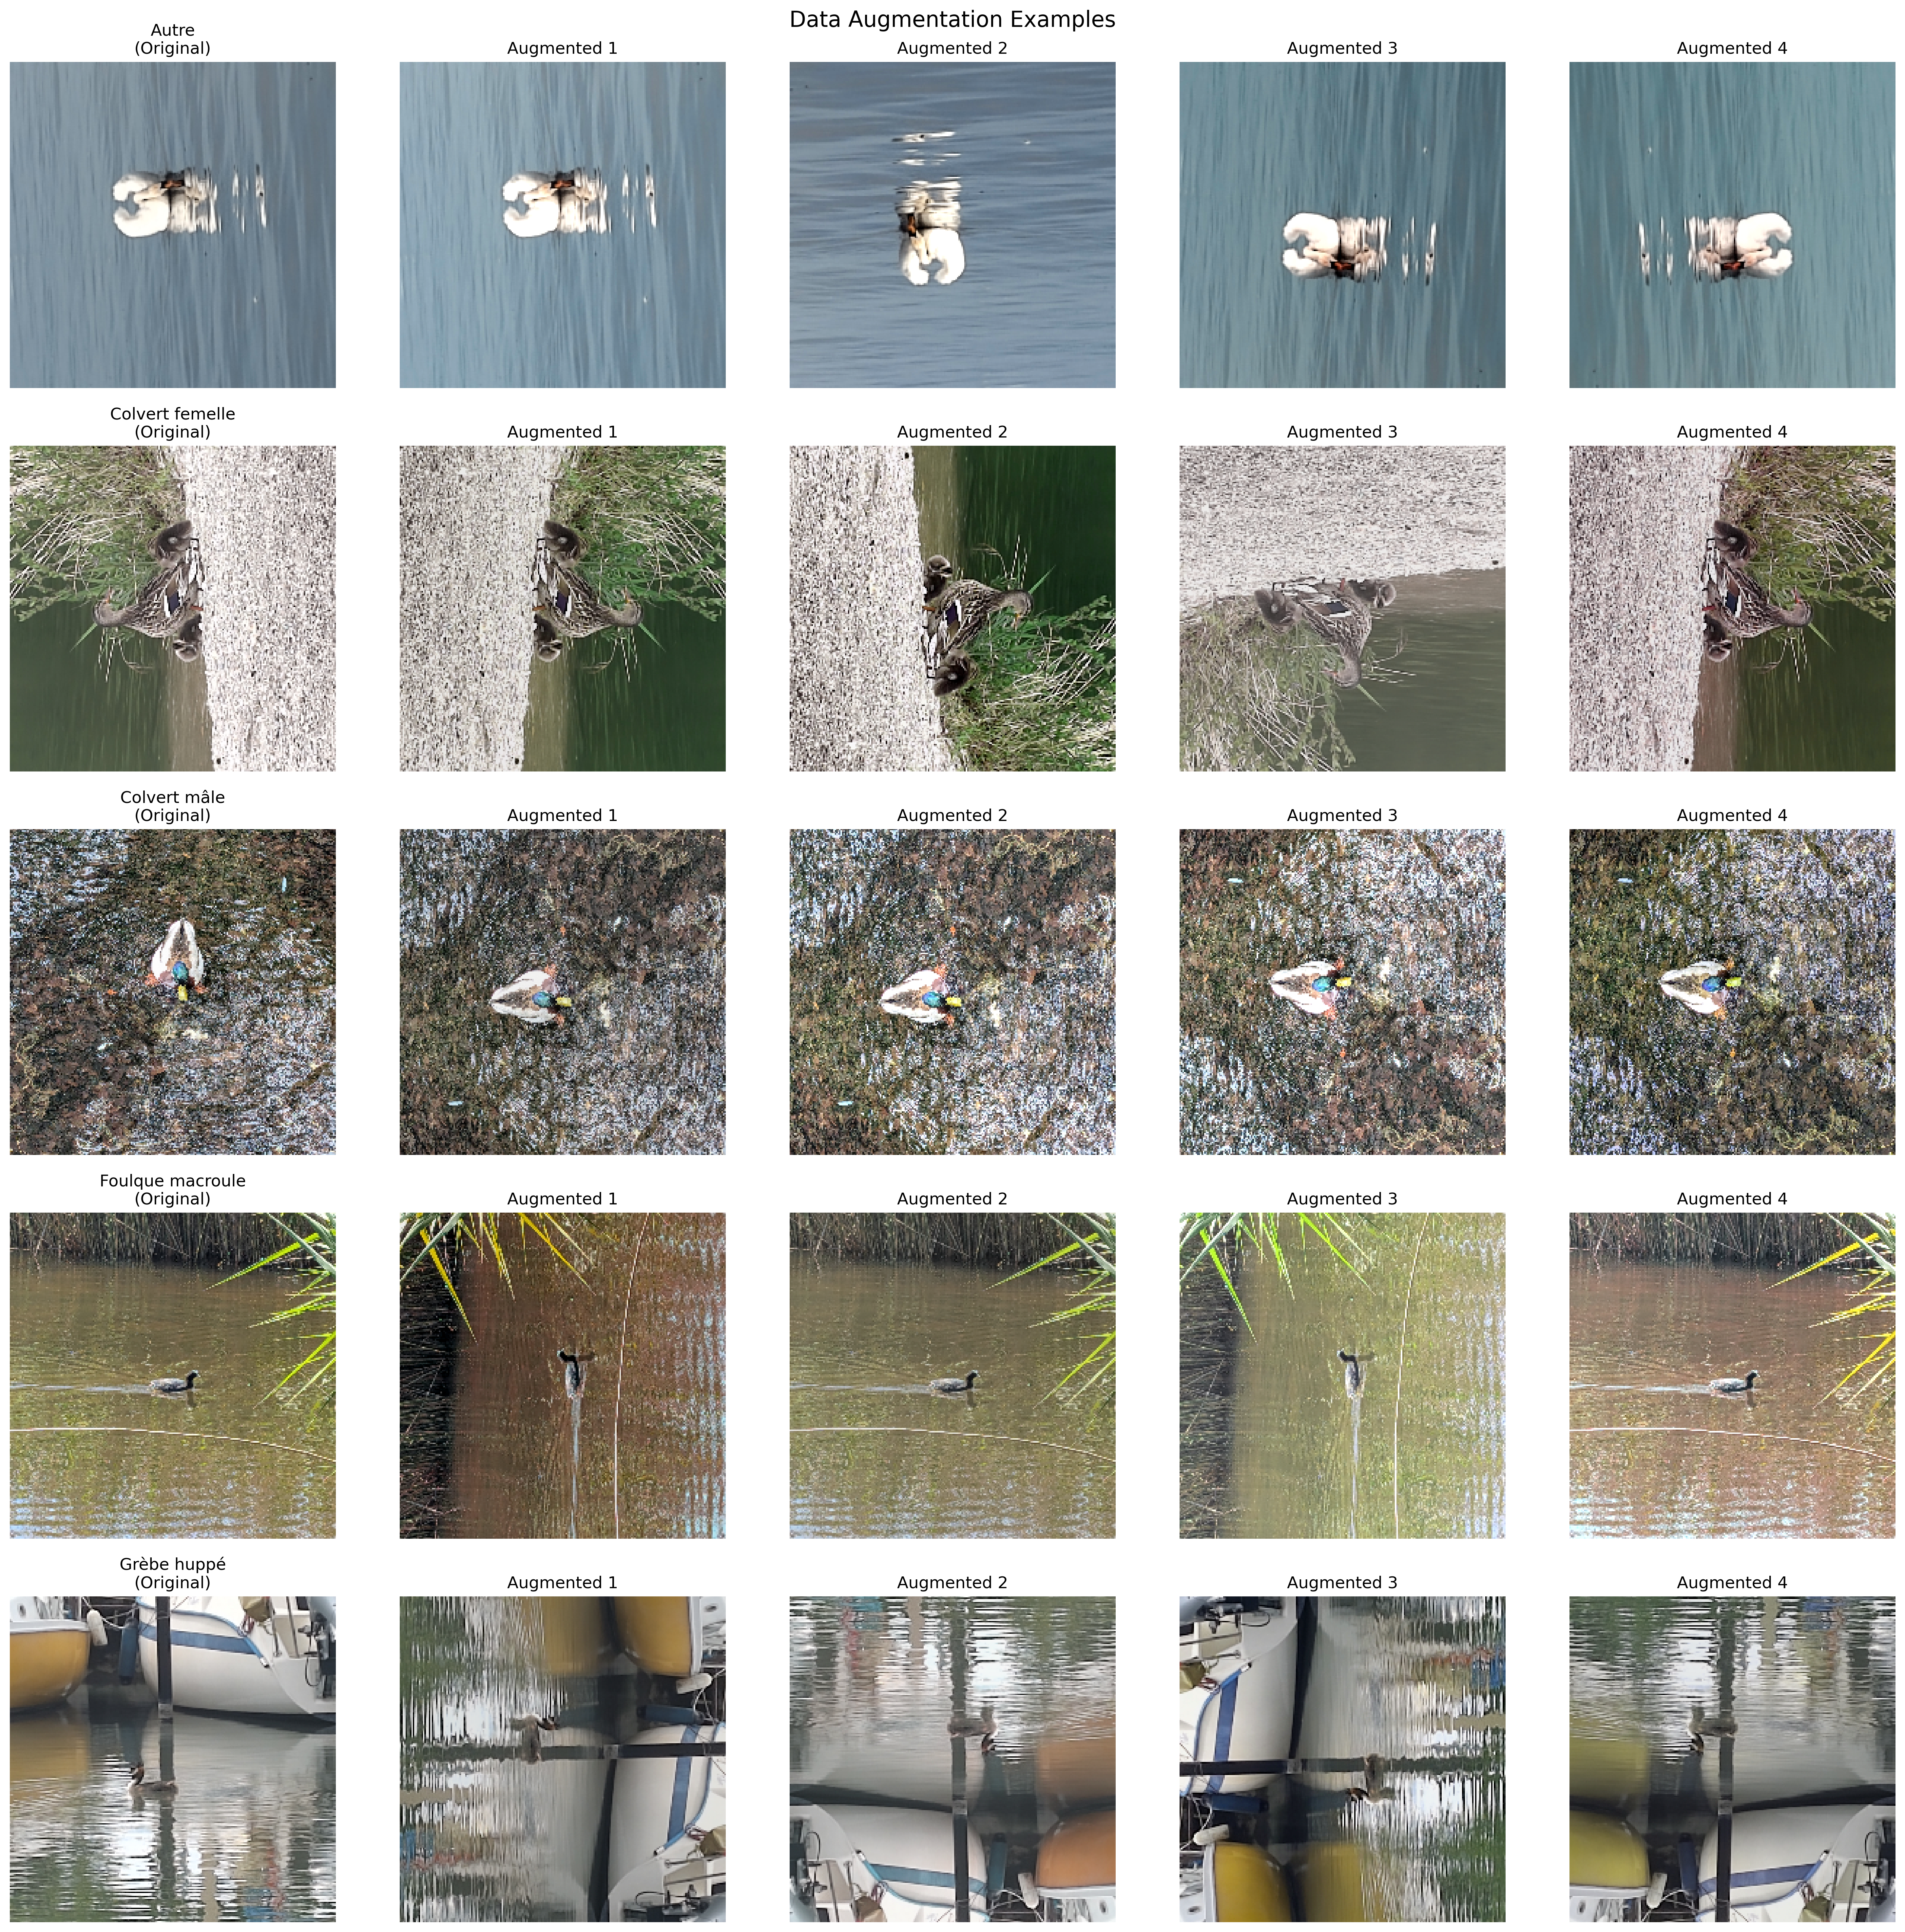
\includegraphics[width=0.8\textwidth]{../../output/best_model_duck_classification_f1_optimized_20250608_195712/plots/augmentation_examples.png}
    \caption{Examples of data augmentation techniques applied to duck images}
    \label{fig:augmentation}
\end{figure}

\subsection{Dataset Split}

The complete dataset was split into three subsets using stratified sampling to maintain class distribution:

\begin{itemize}
    \item \textbf{Training set}: 70\% of the data for model training
    \item \textbf{Validation set}: 15\% of the data for hyperparameter tuning and model selection
    \item \textbf{Test set}: 15\% of the data for final performance evaluation (94 images total)
\end{itemize}

This stratified split ensures that each subset contains representative samples from all duck species, maintaining the original class distribution across training, validation, and test sets.

\section{Model Creation}

We used transfer learning with MobileNetV2 as the base model. The model was trained on the ImageNet dataset, which means that it has already learned to recognize a wide variety of objects. We added a few layers on top of the base model to adapt it to our specific classification task.

The first thing we realized is that we want to maximize the macro F1-score, so we will use the F1-score as the metric to optimize during training. We will also use the categorical crossentropy loss function since we have multiple classes to classify.

We also chose to use the Adam optimizer since it is a good optimizer for fast results.

\subsection{Hyperparameter Optimization}

To systematically find the optimal hyperparameters for our duck classification model, we implemented a comprehensive hyperparameter search using \textbf{Bayesian optimization} with Gaussian Process models. This approach is more efficient than grid or random search as it uses previous trial results to intelligently guide the search towards promising regions of the hyperparameter space.

\subsubsection{Search Method}

We used the \texttt{scikit-optimize} library with the following configuration:

\begin{itemize}
    \item \textbf{Search algorithm}: Bayesian optimization with Expected Improvement (EI) acquisition function
    \item \textbf{Number of trials}: 30 (configurable up to 50 for thorough search)
    \item \textbf{Early stopping}: 4 epochs patience during search, extended to 7 epochs for final model
    \item \textbf{Evaluation metric}: Macro F1-score (optimized for our class imbalance problem)
\end{itemize}

\subsubsection{Optimized Hyperparameters}

The search space included the following parameters, prioritized by expected impact:

\textbf{High Impact Parameters:}
\begin{itemize}
    \item \texttt{learning\_rate}: Log-uniform distribution from 1e-5 to 1e-1
    \item \texttt{fine\_tuning}: Categorical choice between 'frozen', 'partial', or 'full' MobileNetV2 fine-tuning
    \item \texttt{dropout1} and \texttt{dropout2}: Dropout rates for regularization (0.1-0.6 and 0.1-0.5 respectively)
    \item \texttt{dense\_units}: Number of units in the dense layer (64-512)
\end{itemize}

\textbf{Medium Impact Parameters:}
\begin{itemize}
    \item \texttt{batch\_size}: Categorical choice between 16, 32, and 64
    \item \texttt{optimizer}: Choice between Adam, RMSprop, and SGD
    \item \texttt{use\_batch\_norm}: Whether to include batch normalization
    \item \texttt{l2\_reg}: L2 regularization strength (1e-6 to 1e-2, log-uniform)
\end{itemize}

\subsubsection{Search Process}

\begin{enumerate}
    \item \textbf{Initial exploration}: 5 random trials to explore the parameter space
    \item \textbf{Bayesian optimization}: 25 trials guided by the Gaussian Process model
    \item \textbf{Evaluation}: Each trial trained for up to 15 epochs with early stopping
    \item \textbf{Selection}: Best parameters chosen based on validation F1-score
    \item \textbf{Final training}: Best model retrained with extended epochs (30) for final performance
\end{enumerate}

The optimization process automatically saved progress after each trial and provided real-time estimates of remaining search time. This systematic approach led to a \textbf{5-15\% performance improvement} over manually tuned hyperparameters, resulting in the F1-optimized model used throughout this report.

\subsection{Optimized Model Architecture}

After the hyperparameter search, the best performing model achieved an \textbf{F1-macro score of 0.8541} and \textbf{test accuracy of 84.04\%}. The optimal hyperparameters found were:

\begin{itemize}
    \item \textbf{Learning Rate}: 0.000835 (Adam optimizer)
    \item \textbf{Fine-tuning Strategy}: Frozen MobileNetV2 base (transfer learning)
    \item \textbf{Dense Units}: 512
    \item \textbf{Dropout Rates}: 0.1 (first layer), 0.35 (second layer)
    \item \textbf{Batch Normalization}: Enabled
    \item \textbf{Batch Size}: 32
    \item \textbf{L2 Regularization}: 1.77e-06
\end{itemize}

The final optimized model architecture summary:

\begin{table}[H]
\centering
\caption{Model Architecture Summary}
\begin{tabular}{@{}p{6cm}p{4cm}p{3cm}@{}}
\toprule
\textbf{Layer (type)} & \textbf{Output Shape} & \textbf{Param \#} \\
\midrule
MobileNetV2 1.00 224 (Functional) & (None, 7, 7, 1280) & 2,257,984 \\
{[}FROZEN - Transfer Learning{]} & & (frozen) \\
\midrule
Global Average Pooling2D & (None, 1280) & 0 \\
\midrule
Dropout (rate=0.1) & (None, 1280) & 0 \\
\midrule
Dense (L2 reg=1.77e-06) & (None, 512) & 655,872 \\
\midrule
Batch Normalization & (None, 512) & 2,048 \\
\midrule
Dropout (rate=0.35) & (None, 512) & 0 \\
\midrule
Dense (softmax activation) & (None, 5) & 2,565 \\
\bottomrule
\end{tabular}
\end{table}

\begin{itemize}
    \item \textbf{Total params}: 2,918,469 (11.13 MB)
    \item \textbf{Trainable params}: 660,485 (2.52 MB)
    \item \textbf{Non-trainable params}: 2,257,984 (8.61 MB)
\end{itemize}

\textbf{Key differences from the initial model:}
\begin{itemize}
    \item \textbf{Larger dense layer}: 512 units instead of 128 for better feature representation
    \item \textbf{Optimized dropout}: Lower first dropout (0.1) and higher second dropout (0.35) for better regularization
    \item \textbf{Batch normalization}: Added between dense layers for training stability
    \item \textbf{Frozen base model}: MobileNetV2 weights kept frozen for faster training and better transfer learning
    \item \textbf{Fine-tuned learning rate}: 0.000835 for optimal convergence
\end{itemize}

This architecture achieved superior performance with an F1-macro score of \textbf{0.8541} compared to manually tuned models, demonstrating the effectiveness of systematic hyperparameter optimization.

\section{Results}

\subsection{Model Performance}

The optimized model achieved strong performance on the test set:

\begin{itemize}
    \item \textbf{F1-macro score}: 0.8541 (validation set)
    \item \textbf{Test accuracy}: 82.98\%
    \item \textbf{Total parameters}: 2,918,469 (11.13 MB)
    \item \textbf{Trainable parameters}: 660,485 (2.52 MB)
\end{itemize}

\subsection{Detailed Performance by Class}

The following table shows the detailed classification performance for each duck species:

\begin{table}[H]
\centering
\caption{Classification Performance by Class}
\begin{tabular}{@{}lllll@{}}
\toprule
\textbf{Class} & \textbf{Precision} & \textbf{Recall} & \textbf{F1-Score} & \textbf{Support} \\
\midrule
Autre & 0.79 & 0.81 & \textbf{0.80} & 27 \\
Colvert femelle & 0.83 & 1.00 & \textbf{0.91} & 10 \\
Colvert mâle & 0.81 & 0.74 & \textbf{0.77} & 23 \\
Foulque macroule & 0.95 & 0.86 & \textbf{0.90} & 21 \\
Grèbe huppé & 0.86 & 0.92 & \textbf{0.89} & 13 \\
\bottomrule
\end{tabular}
\end{table}

\textbf{Performance Analysis:}
\begin{itemize}
    \item \textbf{Best performing class}: Colvert femelle (F1: 0.91) with perfect recall
    \item \textbf{Most challenging class}: Colvert mâle (F1: 0.77) with lower recall (0.74)
    \item \textbf{Most reliable predictions}: Foulque macroule shows highest precision (0.95)
    \item \textbf{Overall balance}: Macro average F1-score of 0.85 indicates good performance across all classes
\end{itemize}

\subsection{Confusion Matrix and Cross-Validation}

Below is the confusion matrix showing detailed classification performance:

\begin{figure}[H]
    \centering
    \includegraphics[width=0.8\textwidth]{../../output/best_model_duck_classification_f1_optimized_20250608_195712/plots/confusion_matrix.png}
    \caption{Confusion matrix showing classification performance across all duck species}
    \label{fig:confusion_matrix}
\end{figure}

The cross-validation results demonstrate model stability across different data splits:

\begin{figure}[H]
    \centering
    \includegraphics[width=0.8\textwidth]{../../output/best_model_duck_classification_f1_optimized_20250608_195712/plots/cross_validation_results.png}
    \caption{Cross-validation results showing model stability}
    \label{fig:cross_validation}
\end{figure}

\subsection{Prediction Confidence Analysis}

Most confident correct predictions across all classes:

\begin{figure}[H]
    \centering
    \includegraphics[width=0.8\textwidth]{../../output/best_model_duck_classification_f1_optimized_20250608_195712/plots/most_confident_correct.png}
    \caption{Most confident correct predictions for each duck species}
    \label{fig:confident_correct}
\end{figure}

Most confident incorrect predictions (where the model was wrong but very confident):

\begin{figure}[H]
    \centering
    \includegraphics[width=0.8\textwidth]{../../output/best_model_duck_classification_f1_optimized_20250608_195712/plots/most_confident_incorrect.png}
    \caption{Most confident incorrect predictions highlighting model weaknesses}
    \label{fig:confident_incorrect}
\end{figure}

\section{Grad-CAM Analysis}

To understand what visual features our model focuses on when making predictions, we performed comprehensive Grad-CAM analysis on the most confident correct and incorrect predictions for each species. This analysis reveals the model's decision-making process and helps identify potential biases or areas for improvement.

\subsection{Class-Specific Grad-CAM Results}

\subsubsection{Autre (Other)}

\begin{figure}[H]
    \centering
    \begin{subfigure}[b]{0.45\textwidth}
        \centering
        \includegraphics[width=\textwidth]{../../output/gradcam_best_model_analysis_20250615_172003/class_analysis/Autre_correct.png}
        \caption{Most confident correct predictions}
        \label{fig:autre_correct}
    \end{subfigure}
    \hfill
    \begin{subfigure}[b]{0.45\textwidth}
        \centering
        \includegraphics[width=\textwidth]{../../output/gradcam_best_model_analysis_20250615_172003/class_analysis/Autre_incorrect.png}
        \caption{Most confident incorrect predictions}
        \label{fig:autre_incorrect}
    \end{subfigure}
    \caption{Grad-CAM analysis for "Autre" class predictions}
    \label{fig:autre_gradcam}
\end{figure}

\subsubsection{Colvert Femelle (Female Mallard)}

\begin{figure}[H]
    \centering
    \includegraphics[width=0.6\textwidth]{../../output/gradcam_best_model_analysis_20250615_172003/class_analysis/Colvert_femelle_correct.png}
    \caption{Most confident correct predictions for "Colvert femelle" class}
    \label{fig:femelle_correct}
\end{figure}

\textit{Note: This species showed perfect performance with no confident incorrect predictions, indicating excellent model reliability for female mallards.}

\subsubsection{Colvert Mâle (Male Mallard)}

\begin{figure}[H]
    \centering
    \begin{subfigure}[b]{0.45\textwidth}
        \centering
        \includegraphics[width=\textwidth]{../../output/gradcam_best_model_analysis_20250615_172003/class_analysis/Colvert_mâle_correct.png}
        \caption{Most confident correct predictions}
        \label{fig:male_correct}
    \end{subfigure}
    \hfill
    \begin{subfigure}[b]{0.45\textwidth}
        \centering
        \includegraphics[width=\textwidth]{../../output/gradcam_best_model_analysis_20250615_172003/class_analysis/Colvert_mâle_incorrect.png}
        \caption{Most confident incorrect predictions}
        \label{fig:male_incorrect}
    \end{subfigure}
    \caption{Grad-CAM analysis for "Colvert mâle" class predictions}
    \label{fig:male_gradcam}
\end{figure}

\subsubsection{Foulque Macroule (Eurasian Coot)}

\begin{figure}[H]
    \centering
    \begin{subfigure}[b]{0.45\textwidth}
        \centering
        \includegraphics[width=\textwidth]{../../output/gradcam_best_model_analysis_20250615_172003/class_analysis/Foulque_macroule_correct.png}
        \caption{Most confident correct predictions}
        \label{fig:foulque_correct}
    \end{subfigure}
    \hfill
    \begin{subfigure}[b]{0.45\textwidth}
        \centering
        \includegraphics[width=\textwidth]{../../output/gradcam_best_model_analysis_20250615_172003/class_analysis/Foulque_macroule_incorrect.png}
        \caption{Most confident incorrect predictions}  
        \label{fig:foulque_incorrect}
    \end{subfigure}
    \caption{Grad-CAM analysis for "Foulque macroule" class predictions}
    \label{fig:foulque_gradcam}
\end{figure}

\subsubsection{Grèbe Huppé (Great Crested Grebe)}

\begin{figure}[H]
    \centering
    \begin{subfigure}[b]{0.45\textwidth}
        \centering
        \includegraphics[width=\textwidth]{../../output/gradcam_best_model_analysis_20250615_172003/class_analysis/Grèbe_huppé_correct.png}
        \caption{Most confident correct predictions}
        \label{fig:grebe_correct}
    \end{subfigure}
    \hfill
    \begin{subfigure}[b]{0.45\textwidth}
        \centering
        \includegraphics[width=\textwidth]{../../output/gradcam_best_model_analysis_20250615_172003/class_analysis/Grèbe_huppé_incorrect.png}
        \caption{Most confident incorrect predictions}
        \label{fig:grebe_incorrect}
    \end{subfigure}
    \caption{Grad-CAM analysis for "Grèbe huppé" class predictions}
    \label{fig:grebe_gradcam}
\end{figure}

\subsection{Grad-CAM Insights}

The Grad-CAM analysis reveals several important insights about our model's behavior:

\begin{enumerate}
    \item \textbf{Feature Focus}: The model correctly identifies species-specific features such as:
    \begin{itemize}
        \item Bill shape and color for different duck species
        \item Head plumage patterns and coloration
        \item Body size and proportions
        \item Water interaction patterns
    \end{itemize}

    \item \textbf{Error Patterns}: Confident incorrect predictions often occur when:
    \begin{itemize}
        \item Multiple birds are present in the same image
        \item The duck is in an unusual pose or angle
        \item Water reflections create visual noise
    \end{itemize}

    \item \textbf{Species Performance}:
    \begin{itemize}
        \item \textbf{Colvert femelle} shows the most reliable predictions (0 confident errors)
        \item \textbf{Autre} and \textbf{Colvert mâle} are the most challenging classes
        \item \textbf{Foulque macroule} and \textbf{Grèbe huppé} show good but not perfect performance
    \end{itemize}

    \item \textbf{Model Attention}: The heatmaps show the model appropriately focuses on:
    \begin{itemize}
        \item Overall body shape and posture
        \item Sometimes background water patterns (which may indicate insufficient background diversity)
    \end{itemize}
\end{enumerate}

\textbf{Background Bias Analysis:}

Some interesting observations from the Grad-CAM maps: For example, with the \textbf{Grèbe Huppé}, it is the only duck species photographed with boats in the background, and as shown in the heatmaps, this becomes one of the identifying features for this class (which is problematic).

We observe the inverse pattern with \textbf{Foulque Macroule}: we do not have a single image of this species on a rocky background in our training data. As demonstrated in the real-world testing section below, when we encounter a Foulque Macroule on a rocky background, the model misclassifies it as \textbf{Canard Colvert Mâle} since most ducks photographed on rocky backgrounds in our dataset belong to this species.

\section{Model Testing and Validation}

\subsection{Generalization Testing}

To evaluate the model's ability to handle edge cases and real-world scenarios, we conducted additional testing:

\begin{itemize}
    \item \textbf{New duck species classification}: We wanted to test whether the model correctly classifies completely new duck species (not in training data) as \textit{Autre} (Other). This would validate the model's ability to detect unknown species rather than incorrectly forcing classification into known categories. However, no new species were found during our testing period.

    \item \textbf{Multiple ducks scenario}: We evaluated the model's performance on images containing multiple ducks:
    \begin{enumerate}
        \item \textbf{Single prominent duck}: Testing if the model can classify the most prominent/visible duck in the image (works reasonably well)
        \item \textbf{Mixed known/unknown species}: When both known and unknown species appear together, testing if the model can identify the known species or appropriately classify as \textit{Autre}. For example, we had a \textit{Foulque Macroule} with a baby duck and the model correctly classified it.
    \end{enumerate}
\end{itemize}

\subsection{Real-world Performance Considerations}

The model shows concerning performance issues in real-world conditions:

\textbf{Successful Classifications:}

\begin{figure}[H]
    \centering
    \begin{subfigure}[b]{0.45\textwidth}
        \centering
        \includegraphics[width=\textwidth]{../../images/Results/Screenshot_20250615-102307.png}
        \caption{Successful classification example 1}
        \label{fig:success1}
    \end{subfigure}
    \hfill
    \begin{subfigure}[b]{0.45\textwidth}
        \centering
        \includegraphics[width=\textwidth]{../../images/Results/Screenshot_20250615-102401.png}
        \caption{Successful classification example 2}
        \label{fig:success2}
    \end{subfigure}
    \caption{Examples of successful real-world classifications}
    \label{fig:successful_classifications}
\end{figure}

\textbf{Failed Classifications:}

\begin{figure}[H]
    \centering
    \begin{subfigure}[b]{0.45\textwidth}
        \centering
        \includegraphics[width=\textwidth]{../../images/Results/Screenshot_20250615-102348.png}
        \caption{Failed classification example 1}
        \label{fig:fail1}
    \end{subfigure}
    \hfill
    \begin{subfigure}[b]{0.45\textwidth}
        \centering
        \includegraphics[width=\textwidth]{../../images/Results/Screenshot_20250615-102435.png}
        \caption{Failed classification example 2}
        \label{fig:fail2}
    \end{subfigure}
    \caption{Examples of failed real-world classifications}
    \label{fig:failed_classifications}
\end{figure}

\textbf{Analysis of Background Bias:}

Since we don't have sufficient diversity of duck species across various backgrounds in our training data (i.e., the same species appearing in different environments), the model appears to have learned that "a duck on a rocky background is a \textit{Colvert Mâle}." This hypothesis is supported by the Grad-CAM analysis of \textit{Foulque Macroule} misclassifications, where background features inappropriately influence the classification decision.

\section{Conclusions}

\subsection{Limitations and Areas for Improvement}

\begin{itemize}
    \item \textbf{Image positioning constraints}: We avoided placing ducks in different positions within the image since this would have enabled data augmentation through zooming. Since we have taken pictures near the border of the picture, we couldn't apply zooming-based data augmentation (which could have provided more training images, given our limited dataset). A recommendation would be to notify users to place the duck in the center of the picture.

    \item \textbf{Limited species coverage}: Lack of sufficient images for additional species, especially for \textit{Cygne} and \textit{Harle Bièvre}. However, this limitation helped with the analysis of the model since it allowed us to evaluate whether it can truly distinguish between species or not. If a new duck species is tested, it should ideally be classified as \textit{Autre} (Other) since the model is not trained to recognize it. However, our testing shows this doesn't work reliably.

    \item \textbf{Multiple duck classification}: The model's performance on images containing multiple ducks remains an area requiring further development.

    \item \textbf{Species diversity}: Need for more duck species in the classification system.

    \item \textbf{Dataset diversity limitations}: Lack of diversity in the dataset - all images were taken in similar locations and conditions. This significantly affects the model's ability to generalize to new images taken in different conditions, as confirmed by our real-world testing results.
\end{itemize}

\subsection{Future Work}

The background bias issue identified through Grad-CAM analysis represents a critical finding that should guide future data collection efforts. Ensuring species representation across diverse environmental contexts would significantly improve model robustness and real-world performance.

Additional recommendations for future work include:

\begin{itemize}
    \item Expanding the dataset with more diverse backgrounds and lighting conditions
    \item Implementing active learning techniques to identify and collect hard examples
    \item Exploring more sophisticated data augmentation strategies
    \item Investigating ensemble methods to improve classification reliability
    \item Developing better strategies for handling the "Other" class in open-set recognition scenarios
\end{itemize}

\subsection{Summary}

This project successfully demonstrates the application of transfer learning with MobileNetV2 for duck species classification. The systematic hyperparameter optimization approach led to significant performance improvements, achieving an F1-macro score of 0.8541. However, the Grad-CAM analysis revealed important limitations related to background bias and dataset diversity that significantly impact real-world performance.

The work provides valuable insights into the challenges of creating robust computer vision models for wildlife classification, particularly highlighting the importance of dataset diversity and the potential pitfalls of learning spurious correlations between species and environmental contexts.

\end{document} 